\chapter{Design}

\begin{center}
	--- TODO ---
	\begin{itemize}
		\item extended API for SimpleJSON datasource
		\subitem querying available paramaters for a webservice
	\end{itemize}
\end{center}

\section{Architecture}

The designed architecture of the project can be observed in the figure \ref{fig:arch}. There are three data sources connected to Grafana through an extended version of the official SimpleJson data source plugin. Each data source access the data it provides in different ways; through an outside service, from a database or from memory.

\begin{figure}[h]
	\centering
	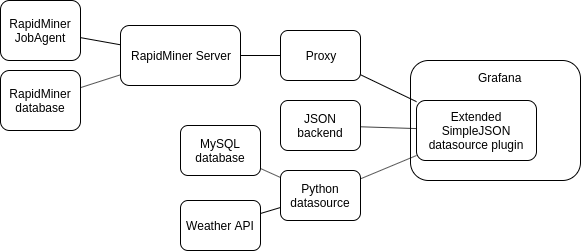
\includegraphics[width=150mm, keepaspectratio]{figures/architecture.png}
	\caption{Architecture diagram}
	\label{fig:arch}
\end{figure}

%---
\section{Components}
%---

In this section, each component is presented, focusing on their responsibilities.

%---
\subsection{Extended SimpleJSON datasource plugin}
%---

Grafana uses data source plugins to connect to different data storage backends. Each data source plugin exposes a Grafana specific interface which allows Grafana to communicate with each data source plugin the same way.


%---
\subsection{Proxy}
%---

The main responsibility of this component is to translate between the RapidMiner Web service which the RapidMiner Server exposes and the SimpleJSON datasource plugin. The problem is that RapidMiner Server exposes its result in JSON, but is in another format that the SimpleJSON datasource plugin accepts.

%---
\subsection{RapidMiner components}
%---
% https://docs.rapidminer.com/latest/server/overview/scalable-architecture.html

The RapidMiner Server acts as a data source for Grafana with the help of the proxy component. In addition to its numerous features, with RapidMiner Server we can store and expose data science processes, like model building, predictions, data ETL operations, etc. Long-running jobs are executed externally via Job Agents. The RapidMiner Server stores its data in an external database.
The Server can expose certain processes that can be called via REST API requests. These are the so called Web services which we use to get the results of the RapidMiner processes and transfer them to Grafana.

%---
\subsection{JSON backend}
%---
% https://github.com/bergquist/fake-simple-json-datasource
This component is a example backend implementation for the SimpleJSON data source plugin. It serves as a base for creating other backends for the data source plugin. It also further expresses the general usability of the SimpleJSON plugin.

%---
\subsection{Python data source}
%---

Although Grafana has a built-in plugin to communicate with a MySQL database, there exists some use-cases, when having a custom component between the data source and the visualization tool is feasible.

With an extra component in the middle, we have extra control over the data which travels from the data storage backend (in our case, MySQL) to the visualization platform. This means that we do not have to rely solely on the capabilities of the database, which can lead to simpler queries, smaller communication overhead with the database.

Having a custom middleware makes it possible to implement the business logic in a separate component and only display business-relevant information with the visualization tool.

It also enables us to aggregate information from different backends and provide only one kind of interface towards visualization which can result in better maintainability.

In this project I demonstrate a proof-of-concept use-case, when this extra components reads information from a database and also from an external API service. I believe, that this is a quite common problem, to have some data in one's storage, but for a better business competence, the usage of external services is also necessary.

%---
\subsection{Weather API}
%---

This component represents the previously mentioned external service. Its responsibility is to expose a service that can be utilized by other softwares in order to acquire additional business-relevant information.

%---
\subsection{MySQL database}
%---

The Python datasource uses this database component to read some sample data from it.


%\begin{itemize}
%	\item why do we need a gateway
%	\item how can we access data from RapidMiner WebService
%	\item why is it good to have a python compoment between Grafana and MySQL
%	\begin{itemize}
%		\item we can customize it better, what we see from the database
%		\item can implement business logic, only see business-relevant projections, granularity of the data
%		\item can aggregate data from different backends
%		\item can aggregate data with outsider APIs (POC implementation for this use-case)
%	\end{itemize}
%\end{itemize}


\begin{itemize}
	\item Grafana
	\item proxy/gateway
	\item python-datasource
	\begin{itemize}
		\item python-datasource
		\item mysql
		\item weather-api
	\end{itemize}
	\item RapidMiner stack
	\begin{itemize}
		\item rapidminer-server
		\item job-agent
		\item database
	\end{itemize}
	\item Grafana datasource plugin (extended API - parameters)
	\begin{itemize}
		\item extended API for asking for available parameters
		\item extended GUI, that dynamically lists available parameters
	\end{itemize}
	\item Grafana extended panel plugin
\end{itemize}